\cotefile{156-4}\scanpage{34}\mspage{33}
% @opening
sous-contrée ; \unsure{Idem} Ce terme est impropre. À moins de réserver le nom de ``contrée'' à \deleted{\uline{tout}} \inserted{\unsure{plus ou moins}} systèmes $(\unsure{\mathcal M|M},\ll,\unsure{\mathcal R|\mathcal Q}_{M})$. Je vais quand $=$ \unsure{réénoncer|r'énoncer} quelques axiomes, \unsure{potentiellement} cruciaux
% @cont1

\uline{Cont} \uuline{1} La relation ``$X\leq Y$'' ($\Longleftrightarrow X\ll Y$ et $X$ comp. $Y$) est une relation d'ordre
% @m1
% slanted
\margin{\uline{\unsure{Cont} 2} Si $X,Y$ sont compatibles, et $X'\leq X$, $Y'\leq Y$ alors $X',Y'$ compatibles}
% @fig2

\deleted{\unsure{Cont 2}} \inserted{\textcircled{\scriptsize Fig 2}} \deleted{\unsure{Toute}} Si $F\in\unsure{\mathcal F|\mathscr F}$, deux éléments \inserted{$X,Y$} de $F$ sont compatibles, et $F$ est une partie \uline{fermée} de l'ens $M(\unsure{\leq|\ll})$.
% @fig3

\deleted{\unsure{Cont 3|Cont 4}} \inserted{\textcircled{\scriptsize Fig 3}} Si $F$ \deleted{et $G$ sont deux} \inserted{est une} figure, \unsure{tte} partie $F'$ de $F$ qui est fermée, est une figure (appelée \uuline{sous-figure}).
% @m2
% slanted
\margin{\uline{NB} Si \deleted{\unsure{$F,G$}} $F',F$ sont des figures telles que $F'\subset F$, alors $F'$ est fermée dans $F$, \unsure{à cause} de Fig 1}
% @empty
% The text enclosed by the long contour is also the conclusion of the lower Cor.
\figure{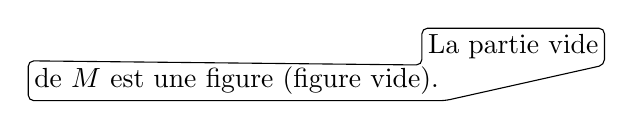
\begin{tikzpicture}[remember picture]
\node[anchor=south west,inner sep=2pt] (emptystart) at (5.0,.20) {La partie vide};
\node[anchor=west,inner sep=2pt] (emptyrest) at (0,0) {de $M$ est une figure (\uuline{figure vide}).};
\draw[rounded corners=2pt] (emptyrest.west) -- (emptyrest.north west) -- (emptystart.south west) -- (emptystart.north west) -- (emptystart.north east) -- (emptystart.south east) -- (emptyrest.south east) -- (emptyrest.south west) -- cycle;
\end{tikzpicture}}
% @fig1

\deleted{\unsure{Cont 3|Cont 4}} \inserted{\textcircled{\scriptsize Fig 1}} Si $X\in M$, l'ens \inserted{$F_{X}=M_{\leq X}$} des \unsure{$Y\in X$} \deleted{tels} \deleted{\unsure{que}} que \unsure{$Y\leq X$} est une figure, qu'on appelle la ``\uuline{figure élémentaire}'' \unsure{définie} par \uline{la} multiplicité $X$.
% @cor

\uline{Cor}. \inserted{(de \unsure{Cont} 2 et \unsure{Cont} 4)} Si $M\neq\varnothing$, \tikz[remember picture,baseline]{\coordinate (corend) at (0,.15); \draw[overlay,->] (emptyrest.west) .. controls +(-1.2,-1.6) and +(-.4,-.8) .. (corend);}
% @nb

\uline{NB} Si $M=\varnothing$, \deleted{Si $M=\varnothing$} l'axiome \uline{Fig \unsure{3|4}} devient vide -- on le remplace par \unsure{:} \deleted{la partie} \deleted{la \unsure{partie vide de|partie vide est} $M$} la seule partie de $M$ (savoir la partie vide) est une figure.
% @cancelled

\deleted{\uline{Cor} (de \uline{Fig 1} et \deleted{\unsure{la}} \uline{Fig 2}) Si \deleted{\unsure{$X$}}, $Y,Z$ sont tels que \unsure{$Y,Z$}$\ll X$, et si $Y,Z$ \unsure{st} comp. à $X$, alors \unsure{sont entre eux}}
\scanpage{35}\mspage{34}
% @old
\deleted{\uline{Contrée finitiste} \unsure{celle} où toute figure}
% @fig

\deleted{\uline{\unsure{Cont 5}}} \inserted{\textcircled{\scriptsize Fig 4}} Soient $F$ et $\unsure{G|C}$ deux figures, telles que pour \unsure{tt} \deleted{$\forall$}$X\in F$, $Y\in G$, $\unsure{x|X}$ et $Y$ comp.
% @side
% slanted
\margin{On dit alors que $F$ et $G$ sont des \uline{figures compatibles}}
% @union
Alors $F\cup G$ est une figure -- \deleted{\unsure{tels}} (\uuline{figure réunion}).
% @meet

Bien sur $F\cap G$ est une sous-figure commune de $F$ et de $G$.
% @oldcor

\deleted{Corollaire (de Fig 1, Fig 2, Fig 4 -- \unsure{renforce|renforcer} le cor. précédent) Si $X,Y,\unsure{x'|X'},\unsure{y'|Y'}$ sont tels que $X'\ll X$, $Y'\ll Y$, et $\{X,Y\}$, $\{X',X\}$, $\{Y',Y\}$ comp., alors $X',Y'$ comp.}
% @fin

\uline{Contrée finitiste} \unsure{Ou|où} les figures sont finies. \deleted{Multistructure finitiste. \unsure{/}} \deleted{\unsure{Une}}
% @cor

\uline{Corollaire} \inserted{(de \uline{Cont} \unsure{2|8}, \uline{Cont} 3, \uline{Cont} 5)} Les figures finies \deleted{sont} exactement les parties \uline{finies} de $M$, fermées pour $\leq$, formées d'é\deleted{\unsure{léments}} \deleted{\unsure{une}} d'é\deleted{\unsure{léments}} \inserted{\unsure{multistés|multisttes}} qui sont mutuellement compatibles.
% @donc

\unsure{Donc}, \deleted{\unsure{la structure} Contrée finitiste} \deleted{\unsure{une}} \inserted{les figures finies} \unsure{se pvt|se pt} \deleted{\unsure{et co}} \unsure{connaître} quand on connaît seulement $\ll,\unsure{\mathcal R|\mathcal Q}_{M}$. \inserted{\unsure{Donc|Dans} une contrée finitiste est \unsure{connue}, par les seules structures $\ll,\mathcal R_{M}$ ;}
% @question
Si on se donne deux telles relations, \inserted{(ordre, et rel. sym. \unsure{réfle.})} satisfaisant \uline{Cont} 1, à quelles conditions les parties finies $\leq$-fermées \deleted{\unsure{que}} et formées d'éléments mut. compatibles (\unsure{i.e|id} les \uline{configurations}) satisf\deleted{\unsure{ass|ais}}ont-elles \uline{Cont} 2 à \uline{Cont} 5, ?
\scanpage{36}\mspage{35}
% @opening
\deleted{\unsure{Il faut que|figure} \unsure{l'on a|On a}} La condition est la suivante ; \deleted{\unsure{qu'on requiert}}
% @fini

\uline{Cont} \deleted{\unsure{2|3}}$3'$ (\unsure{Facultative|Facultatif} dans le cas non finitiste) \deleted{$\forall$} Pour tout $X\in M$, \deleted{la figure} \inserted{l'ens} $M_{\leq X}$ est fini. (i.e. les figures élémentaires sont finies)
% @dims

Par contre, on exige en tous cas que la \uuline{dimension combinatoire} de tout \deleted{\uline{Cont} 3 \unsure{La}} $X\in M$ soit finie (i.e. $\dim\text{ comb }M_{\leq X}$ \unsure{finie}), et plus \deleted{\unsure{géné}} précisément encore
% @mark
% slanted
\margin{\uuline{\unsure{devant|dim ou 1|dim ou I}}\hspace{2pt}\tikz[baseline]{\draw (0,-.2)--(0,.4) (.045,-.2)--(.045,.4) (.09,-.2)--(.09,.4);}}
% @sup
\[
\uline{\text{Cont}}\,3 \quad \text{Si } X\in M,\qquad
\underbrace{\mathop{\mathrm{Sup}}\limits_{X'\ll X}\,\mathrm{dim\,comb}\,M_{\leq X}}_{\text{\uline{dimension} (\unsure{géom}) de }X}<\infty
\]
% @place
On appelle \uuline{lieu} un \unsure{élémt|élément} de $M$ minimal pour $\unsure{\ll|\leq}$. On dénote par $L$
% @subset
\[
L\subset M
\]
% @endplace
l'\unsure{ens} des lieux.
% @shadow

Pour tout $X$, son \uuline{ombre} \inserted{(fermée)} sur $L$ est l'ens $L_{X}$ des lieux $x$ \deleted{$\unsure{\ll X}$} ``de $X$'' i.e. tels que $x\ll X$. On pose
% @sidelf
% slanted
\margin{$L_F=\bigcup_{X\in F}L_X$ s'appelle \uline{l'ombre} de \uline{la} figure \uline{$F$}}
% @lf
\[
L_X^{\unsure{\circ|0}}=L_X\setminus\bigcup_{Y<X}L_Y
\]
% @axiom

\uline{Cont} \deleted{\unsure{5}}4 \quad a) $\forall X\in M$, on a $L_X^{\circ}\neq\varnothing$

% @axiomb
b) Si $X,Y$ sont compatibles et distincts on a
% @disjoint
\[
L_X^{\circ}\cap L_Y^{\circ}=\varnothing
\]
\scanpage{37}\mspage{36}
% @schol
\uline{Scholie} \deleted{L'applicat\unsure{ion}} Soit $\unsure{F|\mathcal F}$ une figure. Alors

% @maponelead
a) L'application
% @mapone
\diagram{\begin{tikzcd}[ampersand replacement=\&,column sep=small]
X\arrow[r,mapsto] \& L_X=\widetilde X \& F\arrow[r,phantom,"{\unsure{\relbar\joinrel\relbar\!\shortmid|\longrightarrow}}" description] \& \unsure{\mathrm P|\mathcal P}(\unsure{L|\mathcal L})
\end{tikzcd}}
% @image
est injective, et son image \inserted{$\widetilde F$} est un ensemble de parties ``\unsure{admissible|admissibles}'' de l'ensemble $L$, i.e.
% @unions
\[
\text{\unsure{a)}}\quad\forall\widetilde X,\widetilde Y\in\widetilde F,\quad\text{on a}\quad
\widetilde X\cap\widetilde Y=\bigcup_{\substack{\widetilde Z\in\widetilde F\\ \widetilde Z\subset\widetilde X\cap\widetilde Y}}\widetilde Z
\]
% @partb
\[
\begin{aligned}
&\text{b)}\quad \forall\widetilde X\in\widetilde F,\quad\text{posant}\quad
\partial\widetilde X=\bigcup_{\substack{\widetilde Y\in\widetilde F\\ \deleted{\unsure{X|Y}}\widetilde Y\subsetneq\widetilde X}}\widetilde Y,\quad\text{et}\\
&\qquad\widetilde X^{\unsure{\circ|0}}=\widetilde X\setminus\partial\widetilde X,\quad\text{on a}\qquad\qquad \widetilde X^\circ\neq\varnothing
\end{aligned}
\]
% @margin
% slanted
\margin{\uline{\unsure{Déf}} La figure $\partial X=\{Y\in M\mid Y<X\}$ s'appelle \uline{le bord} de $X$}
% @name

On \deleted{b) L'application \unsure{$X$}} appelle $\widetilde X^\circ$ l'\uline{ombre ouverte} de $\widetilde X$ sur $L$, $\partial\widetilde X$ \deleted{\uline{l'ombre \unsure{frontière}}} \inserted{\uline{bord d'ombre}}
% @maptwolead

b) L'application
% @maptwo
\diagram{\begin{tikzcd}[ampersand replacement=\&,column sep=small]
X\arrow[r,phantom,"{\unsure{\longmapsto|\mapstochar\relbar\joinrel\relbar}}" description] \& L_X^\circ=\widetilde X^\circ \& F\arrow[r,phantom,"{\unsure{\longrightarrow|\relbar\joinrel\relbar}}" description] \& \mathrm P(L).
\end{tikzcd}}
% @partition
est injective, et \deleted{\unsure{les} de $F$} les images forment une \uline{partition} de l'ombre $L_F$ de la figure $F$, indexée par $F$.
% @order

c) \deleted{\unsure{Soit}} La relation $\leq$ sur $F$ est celle induite par la relation d'inclusion sur les ombres. Si $X\unsure{,|.}Y\in F$, alors conditions \unsure{équiv.}
% @four
\[
\left\{\begin{aligned}
&\text{(i)}\;X\leq Y\\
&\text{(ii)}\;\widetilde X\unsure{\subseteq|\subset}\widetilde Y\\
&\text{(\unsure{iii})}\;\widetilde X^\circ\subseteq\widetilde Y\\
&\text{(iv)}\;\widetilde X^\circ\cap\widetilde Y\neq\varnothing
\end{aligned}\right.
\]
\scanpage{38}\mspage{37}
% @d
d) \deleted{\unsure{Les}} Pour tte sous figure $\unsure{F'|\mathcal F'}$ de $F$, on a \deleted{$\unsure{L_F}$} $\widetilde F'=L_F\subset L$ son ombre, et
% @map
\diagram{\begin{tikzcd}[ampersand replacement=\&]
\unsure{\mathbb F'|F'}\arrow[r] \& \widetilde F'
\end{tikzcd}}
% @bijection
est une bijection de l'ens des sous-figures de $F$, \unsure{avec|sur} l'ens des parties de $\widetilde F$ (ombre de $F$) qui sont ``fermées'' pour le \unsure{rec.} admissible de $\widetilde F$ par \inserted{l'ens.} des $\widetilde X$ ($X\in F$).
% @prop

\uline{Proposition} Soit $M$ une contrée, $M'$ une sous contrée, \deleted{\unsure{on pourrait|on prend}} i.e. une partie de $M$, fermée pour $\ll$, et munie des relations $\underset{M'}{\ll},\unsure{\mathcal R|\mathcal Q}_{M'}$ induites par $M$, et de l'ens \inserted{$\unsure{\mathcal F|\mathrm F}_{M'}$} des parties \deleted{\unsure{$M'$}} \inserted{de $M'$} qui sont des figures de $M$. Alors
% @triple
\[
(M',\underset{M'}{\ll},\mathcal F_{M'})
\]
% @conds
satisfait les conditions \uline{Cont} 1 \unsure{:|à} \uline{Cont} 4, et si $X\in M'$, ses \unsure{dimens|dimm's} combinatoires et géométrique sont les \unsure{$=$s|$\Rightarrow$} dans $M$ et dans $M'$. Si $L'=M'\cap L$, alors pour \deleted{tout} $\mathbb F\in\mathcal F_{M'}$, son ombre \inserted{(fermée)} pour $M$ ou $M'$ est la $=$, si si $X\in M'$, \deleted{\unsure{$X$}} son ombre ouverte est la $=$ \inserted{pour $M$ et pour $M'$}, \unsure{D} $=$ pour le bord $\partial X$. Les conditions Fig 1 \unsure{à|:} Fig 4 sont valables dans $M'$. La condition \uline{Cont} $3'$ \deleted{\unsure{est valable}} est
\scanpage{39}\mspage{38}
% @continuation
également stable par passage à une sous-contrée. Enfin, si $\unsure{C|\mathcal C}$ est finitiste, $\unsure{C'|C}$ aussi\unsure{.|?}
% @disj

\uuline{Figures disjointes} On dit que deux figures sont disjointes si elles sont compatibles, et si leur intersection est vide (\unsure{pas|que} de \unsure{multistrutes|multistructes} communes).
% @warn
% slanted
\margin{\uline{attention} Pour que deux figures (\unsure{$=$|ou} élémentaires) soient disjointes, il \unsure{est} \uline{néc}, mais \deleted{\unsure{pas}} \inserted{néc} \unsure{suffis|suffisant} que leurs ombres soient disjointes (\unsure{c.à.d.} : \unsure{cp paires|cp pour} \unsure{simplifient} pour deux lieux !)}
% @warn2
\margin{\unsure{Si} \deleted{\unsure{de}} elles sont compatibles, \deleted{\unsure{et}} et \unsure{?}}
% @objects
On dit que \inserted{\uline{deux \unsure{multistrutes|multistructures}}} $X,Y$ sont \uline{disjointes} si $F_X,F_Y$ le sont, \inserted{i.e. s'il \unsure{n'existe|est existe} pas de \deleted{\unsure{$X$}} $Z\in M$, avec $Z\leq X,Y$}
% @equiv
% slanted
\margin{ou ce qui revient au $=$, si elles sont comp. et \deleted{l'intersection} \deleted{de leurs} ombres sont disjointes (\unsure{ensemblmt|ensemblistmt})}
% @all
% slanted
\margin{Pour que $F,G$ soient disj., il \unsure{f et s.} que $\forall X\in F$, $Y\in G$, $X$ et $Y$ soient disj.}
% @refine

\deleted{\unsure{Soit} de} \deleted{deux} figures $F,G$, on dit que $F$ \uuline{raffine} $G$ (et on écrit $F\ll G$) si $\forall X\in F,\ \exists Y\in G$ tel que $X\ll Y$. Pour deux figures élémentaires $F_X,F_Y$ cela signifie donc \unsure{simplemt|simplmt} que $X\ll Y$.
% @prop

\deleted{Si $F$ raffine $G$} \uline{Proposition} Pour que $F$ soit une sous-figure de $G$, il \unsure{f et s.} que $F$ raffine $G$, et soit compatible à $G$
% @proof

$\Longrightarrow$ \unsure{trivial}, pour prouver $\Longrightarrow$ on note que \inserted{ds la déf. du raffinement,} $X\ll Y$ \deleted{et} $X$ comp. à $Y$ \deleted{\unsure{et}} \unsure{implique} $X\leq Y$, donc $X\in G$ à cause de Fig 2.
\scanpage{40}\mspage{39}
% @axiom
\uline{Cont} 5 Soient $X\unsure{,|.}Y\in M$, $X$ et $Y$ \uline{disjoints}. Alors pour $X'\ll X$ et $Y'\ll Y$, $X'$ et $Y'$ sont \deleted{disjoints} \deleted{compatibles} disjoints
% @sim
% slanted
\margin{\unsure{S'apparente} à \uline{Cont} 2 (page 33)}
% @cancelone

\deleted{Cela signifie donc $1^\circ$) que $X'$ et $Y'$ sont compatibles et $2^\circ$) qu'il n'existe pas de $Z$ \unsure{tels} que $Z\leq X'$, $Z\leq Y'$}
% @canceltwo

\deleted{Alors $X',Y'$ sont $=$ disjoints, car si on avait \inserted{$Z\in M$ avec} $Z\leq X'$, $Z\leq Y'$, alors on aurait $Z\ll X$,}
% @split

Se décompose en deux

% @splita
\textcircled{\scriptsize a} Sous les condition de Cont 5, $X'$ et $Y'$ \unsure{st} \uline{compatibles}
% @noz

\textcircled{\scriptsize b} \deleted{Si $Z$} $\nexists\ Z\in M$ avec $Z\ll X$, $Z\ll\deleted{X}Y$.
% @ip

(i.e si $X,Y$ compatibles, alors $M_{\leq\unsure{x|X}}\cap M_{\leq Y}=\varnothing$ implique même $M_{\ll X}\cap M_{\ll Y}=\varnothing$)
% @cor

\uline{Cor} Si $\unsure{F|\mathcal F}$ et $\unsure{G|\mathcal G|\mathbb G}$ sont des figures disjointes, alors pour tt raffin\unsure{ement} $F'$ de $F$ et tt raffinement $G'$ de $G$, $F'$ et $G'$ sont disjointes.
% @addcor
% slanted
\margin{\uline{Cor} Pour que deux figures \deleted{\unsure{$F,G$}} $F,G$ soient disjointes, \unsure{il} \unsure{f et s} q. pour \unsure{tous} $x\in\widetilde F,y\in\widetilde G$, q $x$ et $y$ disjoints}
% @remark

\uline{Remarque} Soit $M'$ une sous-contrée. Pour deux figures $F,G$ de $M'$, \deleted{\unsure{leur}} \inserted{ou deux \unsure{multiformes|multiplicités|multistrutes} $X.Y$} dire qu'elles sont disjointes au sens de $M'$ ou de $M$ est pareil, et de $=$ pour la notion que $F$ raffine $G$ Si $M$ satisfait \uline{Cont} 5, $M'$ aussi. \inserted{\unsure{it|it.}\deleted{\unsure{ou|em}} pour \uline{Cont} 6 qui suit}
% @six

\uline{Cont 6} (Facultatif ?) Si $X$ \unsure{et,} $Y\in M$ sont tels que \deleted{$\unsure{\forall}$} $\widetilde X\cap\widetilde Y=\varnothing$ \uuline{et} tout $\unsure{a|x}\in\widetilde X$ est comp. à \deleted{\unsure{tous|tout}} $y\in\widetilde Y$, alors $X$ et $Y$ sont disjoints
% @foot
\margin{\tikz[baseline]{\draw[<->] (0,.68)--(.52,.20); \draw (.58,-.13)--(.58,.30) (.63,-.13)--(.63,.30) (.68,-.13)--(.68,.30); \draw (-.08,-.05) ellipse (.035 and .06); \draw (-.08,-.05)--(-.05,.26);}\,\unsure{avec|i.e.} tt \unsure{elt|tel} $\unsure{\widetilde X|\bar X|x}$ disjoint de tout $y\in\widetilde Y$}
\scanpage{41}\mspage{40}
% @title
\uline{Contrées induites}

% @ind
$1^\circ$) Soit $F$ une figure. Contrée \inserted{induite} $C_F$, \deleted{définie par les} c'est la partie fermée de $M_{\ll}$ engendrée par $F$, i.e. l'ens des $X^{\deleted{\unsure{F|f}}}\in M$ tels que $X$ raffine $F$.
% @lieu
% slanted
\margin{\uline{NB} Lieu des lieux de la contrée $C_F$ n'est autre que l'ombre de $F$}

% @resid
\uline{Contrée résiduelle} C'est la \inserted{sous} contrée $C_{\unsure{\complement|C}F}$ \deleted{\unsure{form|for}} formée des $X$ \inserted{$\in M$} qui sont disjoints de $F$. Par C\deleted{\unsure{on|o}}\unsure{onst|ont}. 5, elle est \deleted{stable} \deleted{pour} fermée dans $M^{\deleted{\unsure{\leq|z}}}_{\ll}$.
% @lieures
% slanted
\margin{\deleted{\unsure{Le|La}} Lieu des lieux de $C_{\complement F}$ est contenu dans $\complement_{\unsure{L}}\widetilde F$, mais ne lui est \deleted{\unsure{égal|néces|pas}} pas \unsure{néc\textsuperscript{t}|néc\textsuperscript{t}.} égal.}

% @fig
\deleted{Cor} Soi\deleted{ent}t $F$ une figure, $G$ une \deleted{\uline{Subdivision}} sous figure. La contrée résiduelle de $F$ dans $G$ est par définition
% @meet
\[
 C_{\deleted{\unsure{G}}F}\cap C_{\complement\deleted{\unsure{F}}G}
\]

% @sub
\uline{Subdivision} Soit $F$ \inserted{$\subset M$} une figure, \deleted{et} On appelle \uline{subdivision} de $F$ une figure\unsure{\textsuperscript{o}|.} $F'\subset M$ telle que
% @a

a) $F'$ soit un raffinement de $F$
% @b

b) $F'$ soit maximale \inserted{pour $\subset$}, parmi les \deleted{\unsure{raffi|raffin}} figures qui raffinent $F$.
% @nb

\uline{NB} Si $F'$ raffine $F$, alors son ombre $\widetilde F'$ est contenue dans celle $\widetilde F$ de $F$.
